\documentclass[tikz,border=2pt]{standalone}
\usepackage{amsmath,amssymb}
\usepackage{pgfplots}
\pgfplotsset{compat=1.18}
\usetikzlibrary{arrows.meta}
\begin{document}
% P(M <= z) = G_N(F_X(z)) with N ~ Poisson(5): the PGF e^{-5(1-p)} evaluated at p = F_X(z);
% at p = 0.9 (one claim exceeds 1000 with probability 0.1) it gives e^{-0.5} ~ 0.607; at p = 0 it is P(N=0) = e^{-5}.
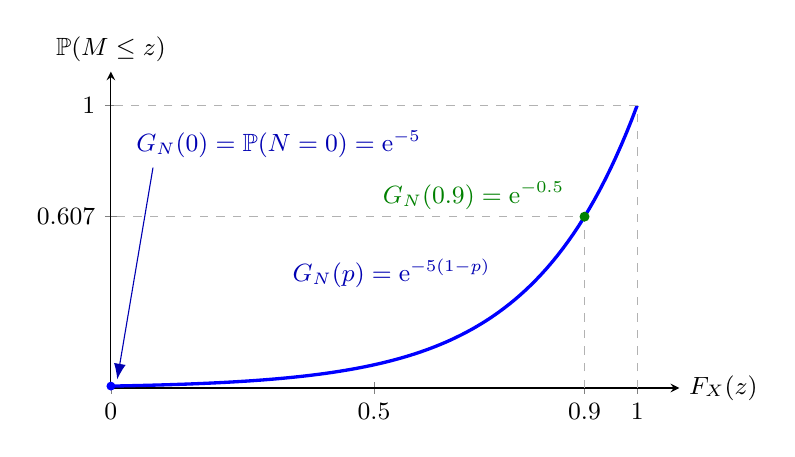
\begin{tikzpicture}[font=\small, >={Latex[length=2mm]}]
  \begin{axis}[
    axis lines=left, xmin=0, xmax=1.08, ymin=0, ymax=1.12,
    xtick={0,0.5,0.9,1}, xticklabels={$0$,$0.5$,$0.9$,$1$}, ytick={0.607,1}, yticklabels={$0.607$,$1$},
    xlabel={$F_X(z)$}, ylabel={$\mathbb{P}(M\le z)$},
    xlabel style={at={(axis description cs:1,0)}, anchor=west},
    ylabel style={rotate=-90, at={(axis description cs:0,1)}, anchor=south},
    samples=100, width=8.8cm, height=5.6cm, clip=false]
    \addplot[blue, very thick, domain=0:1] {exp(-5*(1-x))};
    \draw[gray!60, thin, dashed] (axis cs:0.9,0) -- (axis cs:0.9,0.6065) -- (axis cs:0,0.6065);
    \draw[gray!60, thin, dashed] (axis cs:1,0) -- (axis cs:1,1) -- (axis cs:0,1);
    \fill[green!50!black] (axis cs:0.9,0.6065) circle (1.8pt);
    \node[green!50!black, anchor=east] at (axis cs:0.88,0.68) {$G_N(0.9)=\mathrm{e}^{-0.5}$};
    \fill[blue] (axis cs:0,0.0067) circle (1.6pt);
    \draw[blue!70!black, ->] (axis cs:0.08,0.78) -- (axis cs:0.012,0.03);
    \node[blue!70!black, anchor=south west] at (axis cs:0.03,0.78) {$G_N(0)=\mathbb{P}(N=0)=\mathrm{e}^{-5}$};
    \node[blue!70!black, anchor=south east] at (axis cs:0.74,0.32) {$G_N(p)=\mathrm{e}^{-5(1-p)}$};
  \end{axis}
\end{tikzpicture}
\end{document}
